\documentclass[10pt, a4paper, twosize]{article}
%\documentclass[12pt, a4paper, twoside]{book}

\usepackage{helvet}
\usepackage{hyperref}
\usepackage{graphicx}
\usepackage{listings}
\usepackage{textcomp}
\usepackage[
	a4paper,
	outer=2cm,
	inner=4cm,
	top=2cm,
	bottom=2cm
]{geometry}
\usepackage{float}
\usepackage{tabularx}
\usepackage[disable]{todonotes}
\usepackage{color, soul}
\usepackage{amsmath}
\usepackage{algorithmicx}
\usepackage[noend]{algpseudocode}
\usepackage{algorithm}
\usepackage{framed}
\usepackage{subcaption}
\usepackage{titlepic}
\usepackage{fancyhdr}
\usepackage[simplified]{styles/pgf-umlcd}
\usepackage{shorttoc}
\usepackage{url}
\usepackage{paralist}

\definecolor{grey}{rgb}{0.9, 0.9, 0.9}
\definecolor{dkgreen}{rgb}{0,0.6,0}
\definecolor{dkred}{rgb}{0.6,0,0.0}

\lstdefinestyle{DOS}
{
    backgroundcolor=\color{black},
    basicstyle=\scriptsize\color{white}\ttfamily,
    stringstyle=\color{white},
    keywords={}
}

\lstdefinestyle{makefile}
{
    numberblanklines=false,
    language=make,
    tabsize=4,
    keywordstyle=\color{red},
    identifierstyle= %plain identifiers for make
}

\lstset{
  language=Java,                % the language of the code
  basicstyle=\footnotesize\ttfamily,
  numbers=left,                   % where to put the line-numbers
  stepnumber=1,                   % the step between two line-numbers. If it's 1, each line
  numbersep=5pt,                  % how far the line-numbers are from the code
  backgroundcolor=\color{white},      % choose the background color. You must add \usepackage{color}
  showspaces=false,               % show spaces adding particular underscores
  showstringspaces=false,         % underline spaces within strings
  showtabs=false,                 % show tabs within strings adding particular underscores
  frame=single,                   % adds a frame around the code
  rulecolor=\color{black},        % if not set, the frame-color may be changed on line-breaks within not-black text (e.g. comments (green here))
  tabsize=2,                      % sets default tabsize to 2 spaces
  captionpos=b,                   % sets the caption-position to bottom
  breaklines=true,                % sets automatic line breaking
  breakatwhitespace=false,        % sets if automatic breaks should only happen at whitespace
  keywordstyle=\color{blue},          % keyword style
  commentstyle=\color{dkgreen},       % comment style
  stringstyle=\color{dkred},         % string literal style
  columns=fixed,
  extendedchars=true,
  frame=single,
}

%\renewcommand{\chaptername}{Topic}

% New definitions
\algnewcommand\algorithmicswitch{\textbf{switch}}
\algnewcommand\algorithmiccase{\textbf{case}}
\algnewcommand\algorithmicassert{\texttt{assert}}
\algnewcommand\Assert[1]{\State \algorithmicassert(#1)}%
% New "environments"
\algdef{SE}[SWITCH]{Switch}{EndSwitch}[1]{\algorithmicswitch\ #1\ \algorithmicdo}{\algorithmicend\ \algorithmicswitch}%
\algdef{SE}[CASE]{Case}{EndCase}[1]{\algorithmiccase\ #1}{\algorithmicend\ \algorithmiccase}%
\algtext*{EndSwitch}%
\algtext*{EndCase}%

\pagestyle{fancy}
\fancyhf{}
\fancyhead[RO, LE]{\small \rightmark}
\fancyfoot[RO, LE]{\small \thepage}

\begin{document}

%\frontmatter

\begin{titlepage}
\vspace*{5cm}
\begin{center}

\includegraphics[width=.5\textwidth]{images/EdNapUniLogoCMYK}~\\[1cm]

\textsc{\Large Edinburgh Napier University}\\[1.5cm]

\textsc{\LARGE \bfseries SET08101 Web Tech}\\[0.5cm]

\hrulefill \\[0.4cm]
{\huge \bfseries Lab 6 - The Server Side \\[0.4cm] }
\hrulefill \\[1.5cm]

\begin{minipage}{0.4\textwidth}
\begin{flushleft} \large
\textbf{Dr Simon Wells} \\
\end{flushleft}
\end{minipage}

\vfill

\end{center}
\end{titlepage}

%\shorttoc{Overview}{0}

%\setcounter{tocdepth}{2}
%\cleardoublepage
%\tableofcontents
%\listoffigures
%\listofalgorithms
%\addtocontents{toc}{~\hfill\textbf{Page}\par}

%\mainmatter

%\input{sections/labs/04_ui}

\section{Aims}
\paragraph{} At the end of the practical portion of this topic you will:

\begin{itemize}
\item deploy your web pages to a web server
\item deploy you web pages to GitHub
\item be aware of the range of paid for services for hosting
\end{itemize}


%\begin{framed}
%{\bf{NOTICE:}  }
%\end{framed}


\section{Activities}
\paragraph{} First we'll find out a bit more about web servers and run one locally to host the pages we've developed so far. Then we'll see how GitHub can be used to host our webpages. Finally, we'll look at the range of online services available to host our web sites.

\subsection{Web Servers}
\paragraph{} So far we've developed some web pages and sites on our local machine then opened them using a web browser on the same machine. This is a perfectly fine way to go about things, particularly early in the development cycle. An awful lot of websites will run from a folder on your local machine. As a rule anything that doesn't rely on additional software, such as a database, or on server side data processing, such as social features or relaying data to other users, will run just fine in the browser. It's only when we need the server to do some processing for us, which takes the load away from our web browser, or when we need to share data, or when we want our pages to be made available to other that we need to get them off our local machine.

\paragraph{} If you are on a lab machine\emph{If you're on a Mac then you can install nginx using homebrew. If you're using Linux then apt-get install nginx (or the equivalent for your distro.)} you can download the latest zipped version of the nginx web server from here: \url{http://nginx.org/download/nginx-1.13.8.zip}.

\paragraph{} Create a folder on your h: drive called ``apps'' and copy your nginx zip to it. Right click on the zip and select ``Extract All...'' from the menu. This should give you a folder called nginx-1.13.8 which you should navigate into. Now open the nginx.conf which can be found in the conf sub-directory. We need to make one tiny alteration here. We need to tell nginx which port to listen on for connections from web browsers. By default nginx will listen on port 80 but this is a \emph{privleged port} which means that you need to be an admin to use it. Instead we are going to use port 5000 which has been made available in the labs for us to use. Line 36 of nginx.conf will contain a line like this:
\begin{lstlisting}[style=DOS]
listen       80;
\end{lstlisting}

\paragraph{} and we need to change it to:

\begin{lstlisting}[style=DOS]
listen       5000;
\end{lstlisting}

\paragraph{} Save nginx.conf and close the file. We can now doubleclick nginx.exe and run our server. 

\begin{figure}[H]
\centering
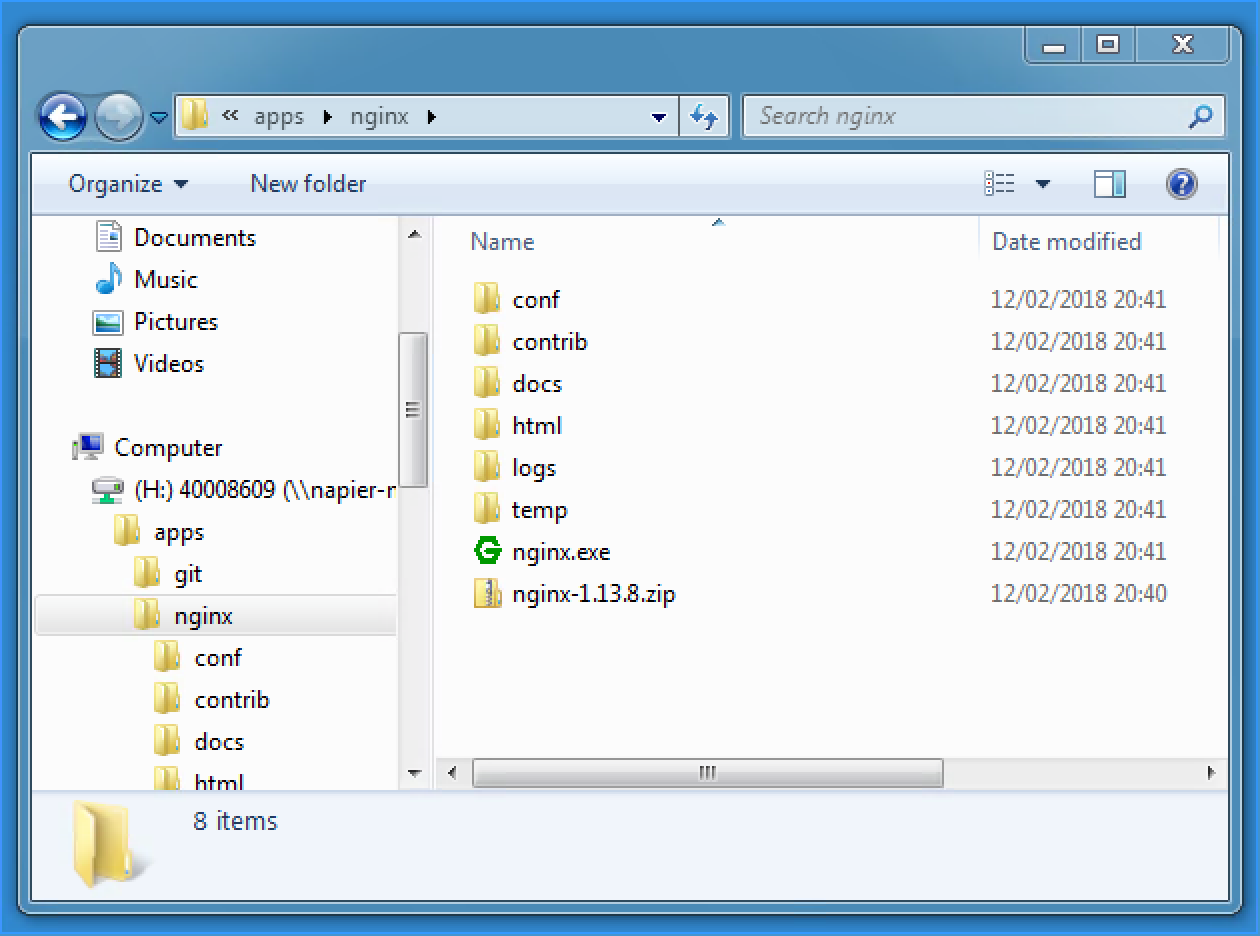
\includegraphics[width=0.85\textwidth]{images/nginx_exe}
\caption{The nginx executable.}
\label{fig:nginx_welcome}
\end{figure}


\paragraph{} There might be some messages from the Windows firewall which you should click through to allow nginx to run. You can now open a browser and navigate to \url{http://localhost:5000}. You should see something similar to the following:

\begin{figure}[H]
\centering
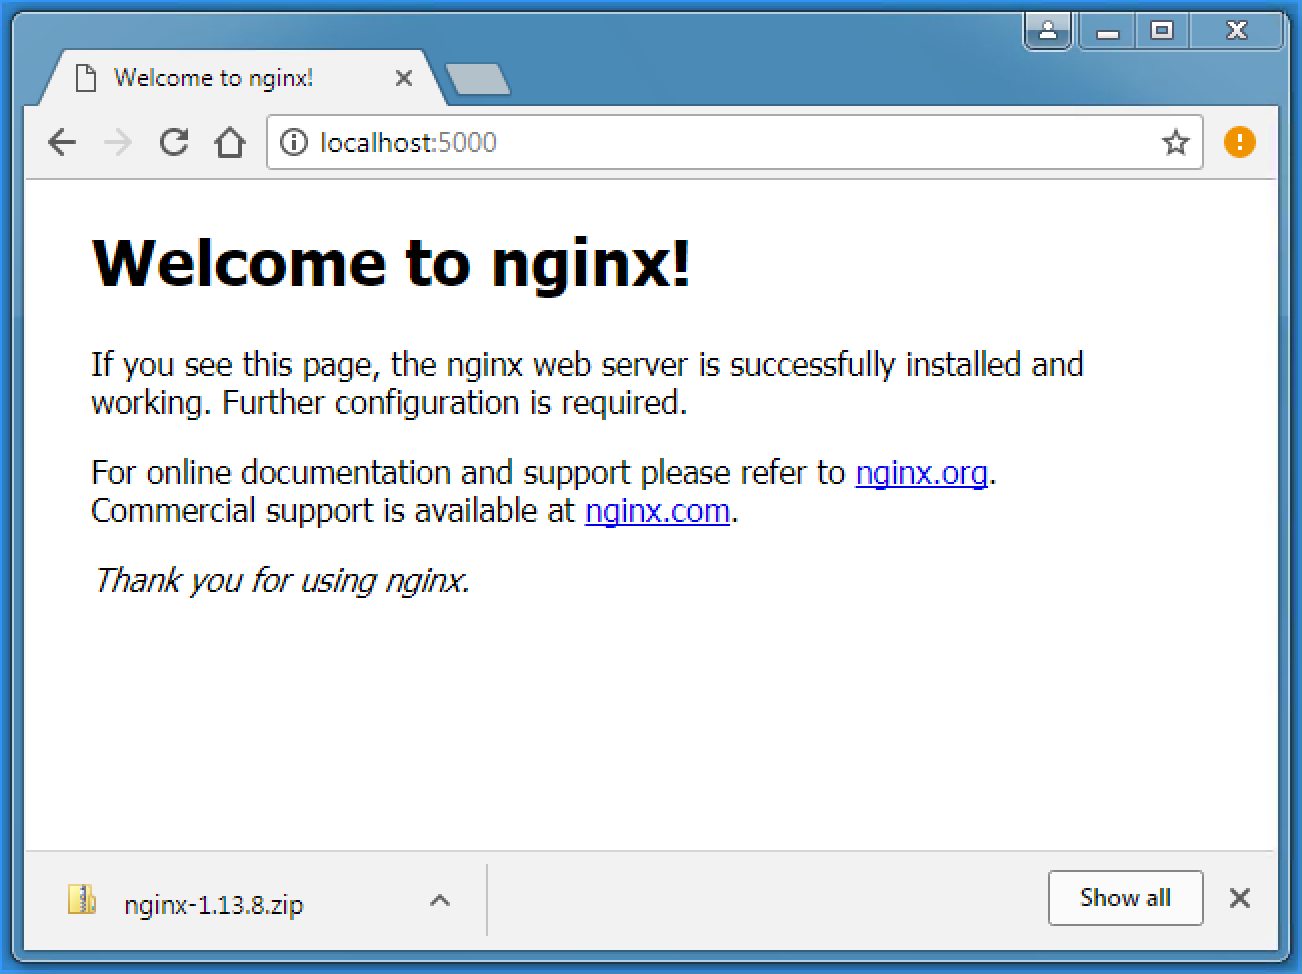
\includegraphics[width=0.85\textwidth]{images/nginx_welcome}
\caption{The default nginx web page at \url{http://localhost:5000}.}
\label{fig:nginx_welcome}
\end{figure}

\paragraph{} The pages that nginx runs can be found in the html subfolder of the nginx folder\footnote{This location will very likely be different if you've installed nginx on a mac or Linux system so you might have to do a little research to get things working properly there. Windows packages things up a bit differently.}. Lets create a quick new HTML file in the html folder and see our page displayed. 

\begin{figure}[H]
\centering
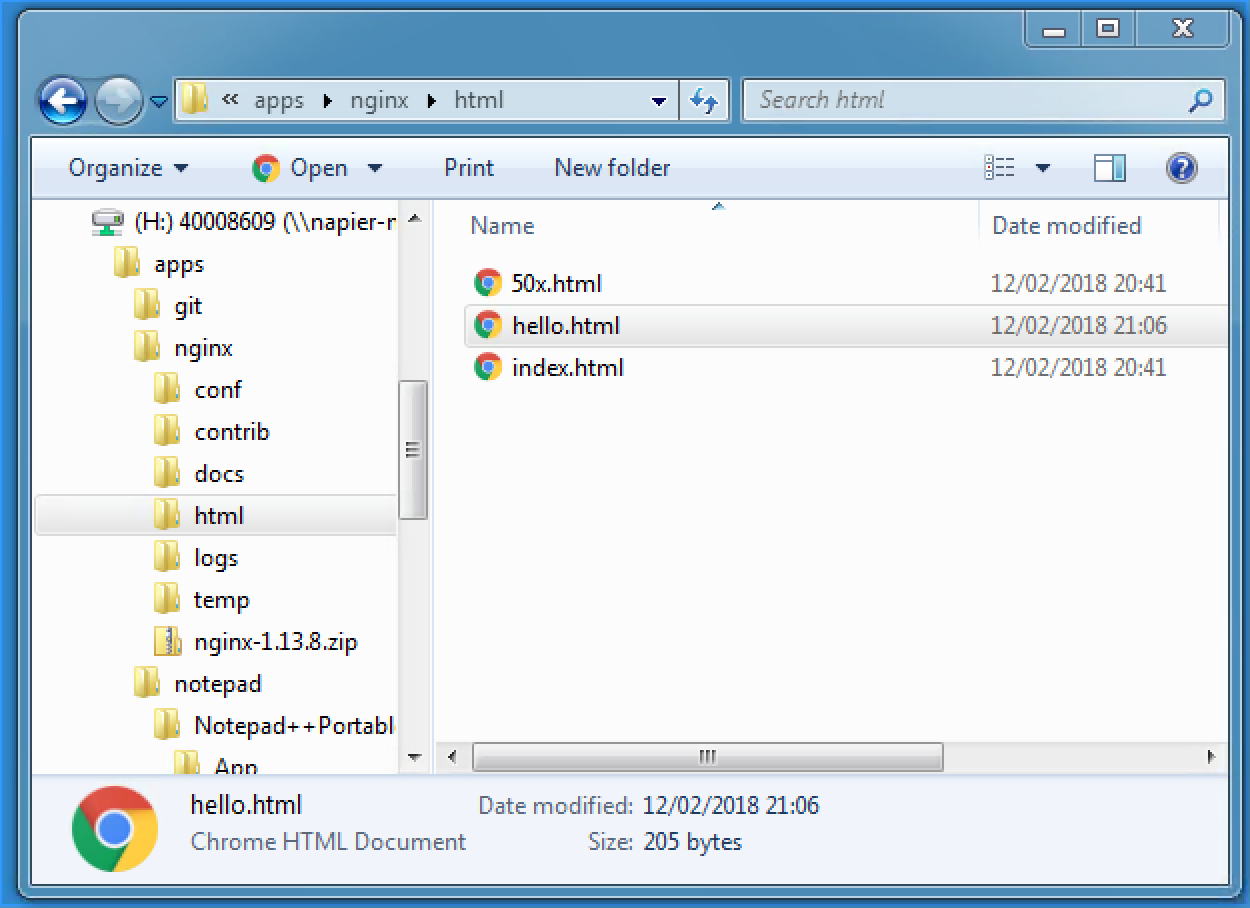
\includegraphics[width=0.85\textwidth]{images/nginx_html}
\caption{Our hello.html file in the nginx html subfolder.}
\label{fig:nginx_welcome}
\end{figure}


\paragraph{} We now need to edit hello.html as follows:

\begin{lstlisting}
<!DOCTYPE html>
<html>
<head>
<title>Hello Napier</title>
</head>
<body>
<h1>Your first page</h1>
<p>Well, kind of. It's (probably [possibly?]) your first page running in a web-server.</p>
</body>
</html>
\end{lstlisting}

Now we can visit \url{http://localhost:5000/hello.html} to see our glorious new page running in a web browser and being served by an actual web server. You should see something like this:

\begin{figure}[H]
\centering
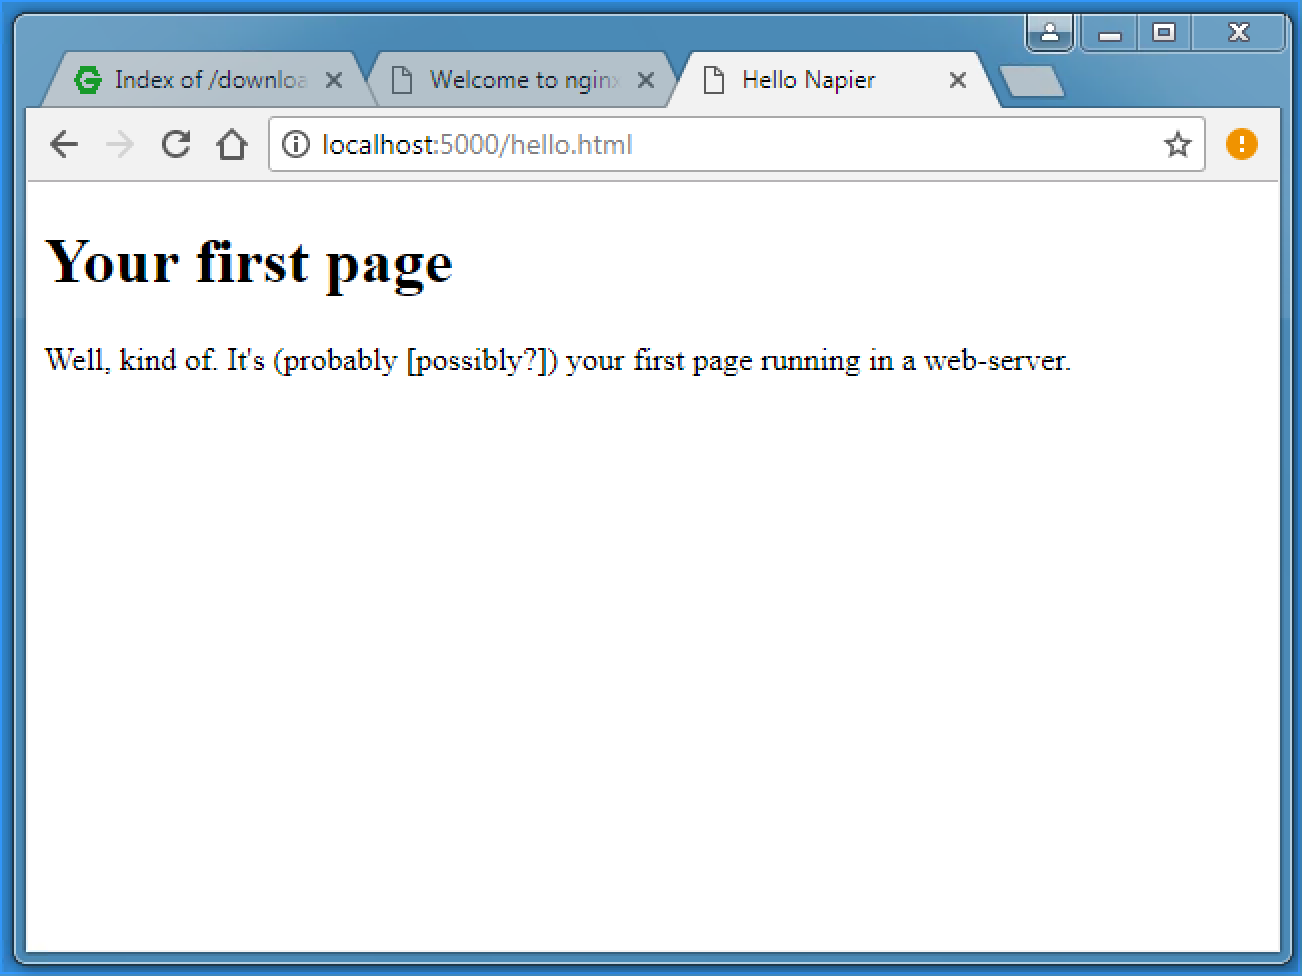
\includegraphics[width=0.85\textwidth]{images/nginx_hello}
\caption{Our ``hello napier'' web page served up by nginx at \url{http://localhost:5000/hello.html}.}
\label{fig:nginx_welcome}
\end{figure}

\paragraph{} Note that we had to specify which file the browser needed to retrieve. Servers will generally serve up an index.html file by default if no other file is explicitly requested. However, the configuration for most web servers will allow you to alter this behaviour if you have a pressing need. In fact, servers can generally be configured and tuned to suit a wide array of situations and needs. However, for now, we don't need to worry too much about tuning our server as it is a really big topic and overlaps very heavily with more general server administration which is concerned with security, reliability, and performance\footnote{This is one of those areas where you can do some background reading but be prepared for a \emph{deep} rabbit hole with the side effect of developing some really useful professional skills.}.

\paragraph{} You can add additional subfolders to the html folder for each of your projects for the moment. Try this and add some of the sites and files that you've been developing in earlier labs. Navigate to your files and compare them to how they look when loading from the file system. Really you shouldn't notice any difference from the user perpsective.

\paragraph{} In reality we would add configuration files for nginx so that the server would listen for requests to various web addresses, for example, the same web server could host many different web sites, each with a different URL. However, like everything else in web land, this is another rabbit hole that you should explore yourself if you want to deploy your own web site on your own server. For the purposes of this lab we'll use the default configuration.

\paragraph{} An important point to note is that our pages are now being server by a real web server. With network and configuration changes\footnote{which we cannot make for security reasons} we could make our nginx server listen for connections from anywhere else on the Internet, and in response, nginx would send back our HTML, CSS, \& JS. There is no real difference, bar some configuration, between what you now have running and many web sites that are out there in the real world. The web really does have quite a low barrier to entry doesn't it. Relate this back to our discussions about how the web is a tool for democratising information and think about how powerful this idea is. \emph{Anyone can run a web server and serve up whatever information they like to whomever wants to read it}.

\paragraph{} It's worth doing some reading about the nginx project, especially if you want to deploy your sites elsewhere than your lab machine. Remember however that nginx is just one, albeit quite popular, web server. There are many others available. For many years Apache was the most popular web server. Ultimately, which server you choose to use will depend upon your expeience and the specific needs of the project that you are working on. Some servers have different capabilities, can work with different sets of server side languages or have different performance characteristics. Nginx for example is currently regarded as relatively fast and efficient for general web site hosting and is also capable of being tuned to scale greatly.

\paragraph{} When you're done playing with nginx you can shut it down using the Windows Task Manager. Press ctrl+shit+escape then look for nginx.exe * 32 in the `Processes' tab. There may be two entries, so select one then click the end process button, then select the other and repeat the process. On a real, public web server we would usually have helper scripts to manage this process but to be honest, we are usually concerned mostly with keeping nginx running constantly rather then starting it up and shutting it down frequently.

\subsection{Hosting Services}
\paragraph{} There are many hosting services that give you free or low-cost \emph{static} hosting. In fact Github actually does this. Any Github repo can serve up html, css, and javascript from a `docs' folder. You just have to configure the repository to do so. For example, my personal web site at \url{https://www.simonwells.org} is actually hosted at GitHub as is the SET08101 websites at \url{https://siwells.github.io/set08101/}.

\paragraph{} If you've a GitHub account then log in and create a new repository. If you haven't got a GitHub account then create one. Clone your new repository and add a new folder called `docs' then put an index.html into the docs folder. Edit the index.html as follows:

\begin{lstlisting}
<!DOCTYPE html>
<html>
<head>
<title>GitHub Hosting</title>
</head>
<body>
<h1>Your first GitHub hosted page</h1>
<p>Some stuff....</p>
</body>
</html>
\end{lstlisting}

\paragraph{} Add, commit, and push your changes to GitHub. Now go to the GitHub repository and check that you docs folder and index.html are there. Now hit the `Settings' button which looks like this:

\begin{figure}[H]
\centering

\includegraphics[width=0.5\textwidth]{images/github_settings}
\caption{The GitHub repository settings button.}
\label{fig:github_settings}
\end{figure}

\paragraph{} Now navigate down to the section named `GitHub' Pages which looks like this:

\begin{figure}[H]
\centering
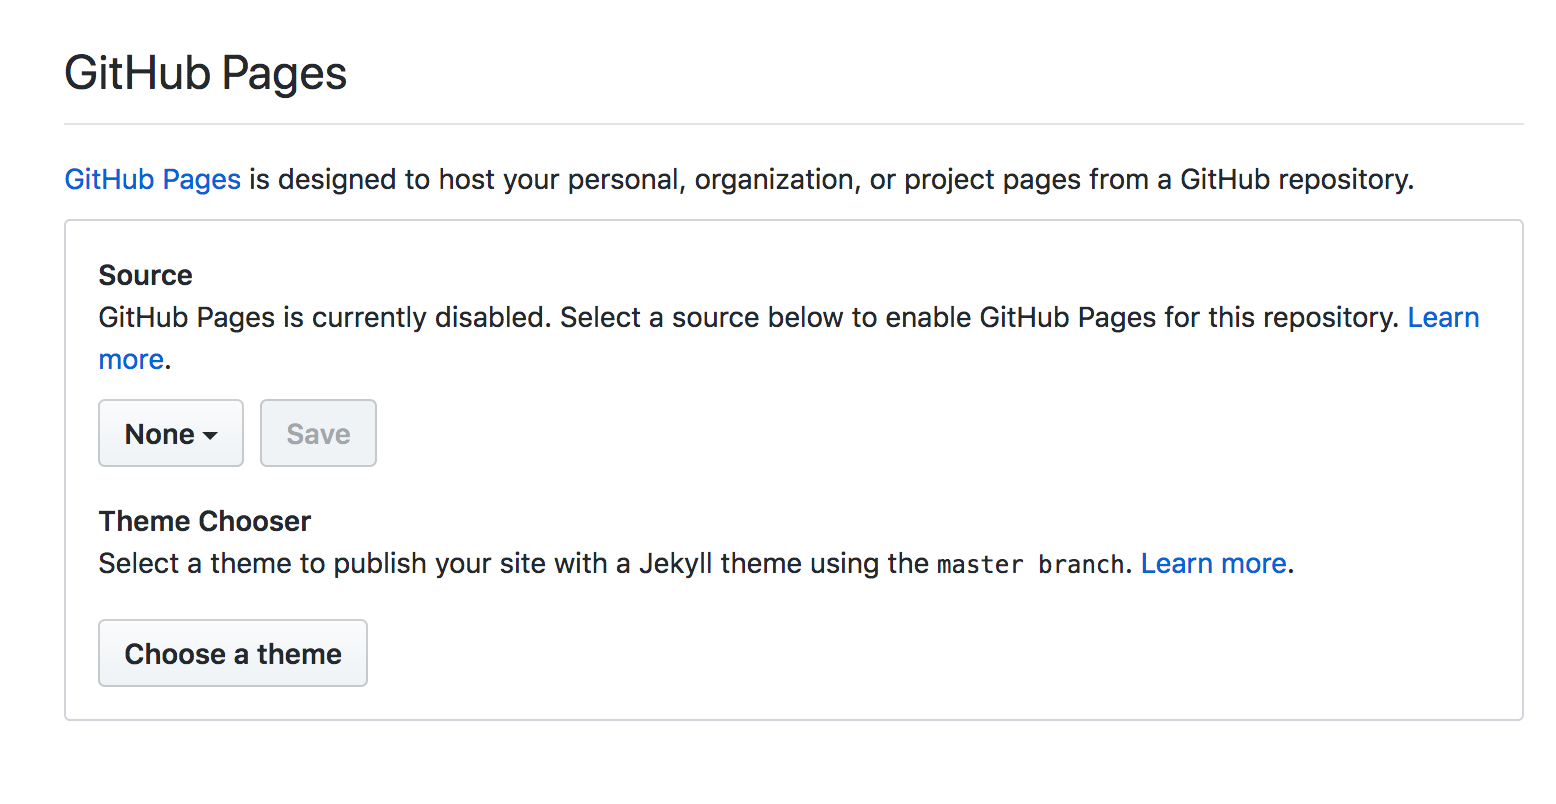
\includegraphics[width=0.85\textwidth]{images/github_config_before}
\caption{The GitHub config page before you enable pages.}
\label{fig:github_config_before}
\end{figure}

\paragraph{} In the drop down select `master branch /docs folder' then hit the save button. If you scroll to the GitHub Pages section again it should look like this:

\begin{figure}[H]
\centering
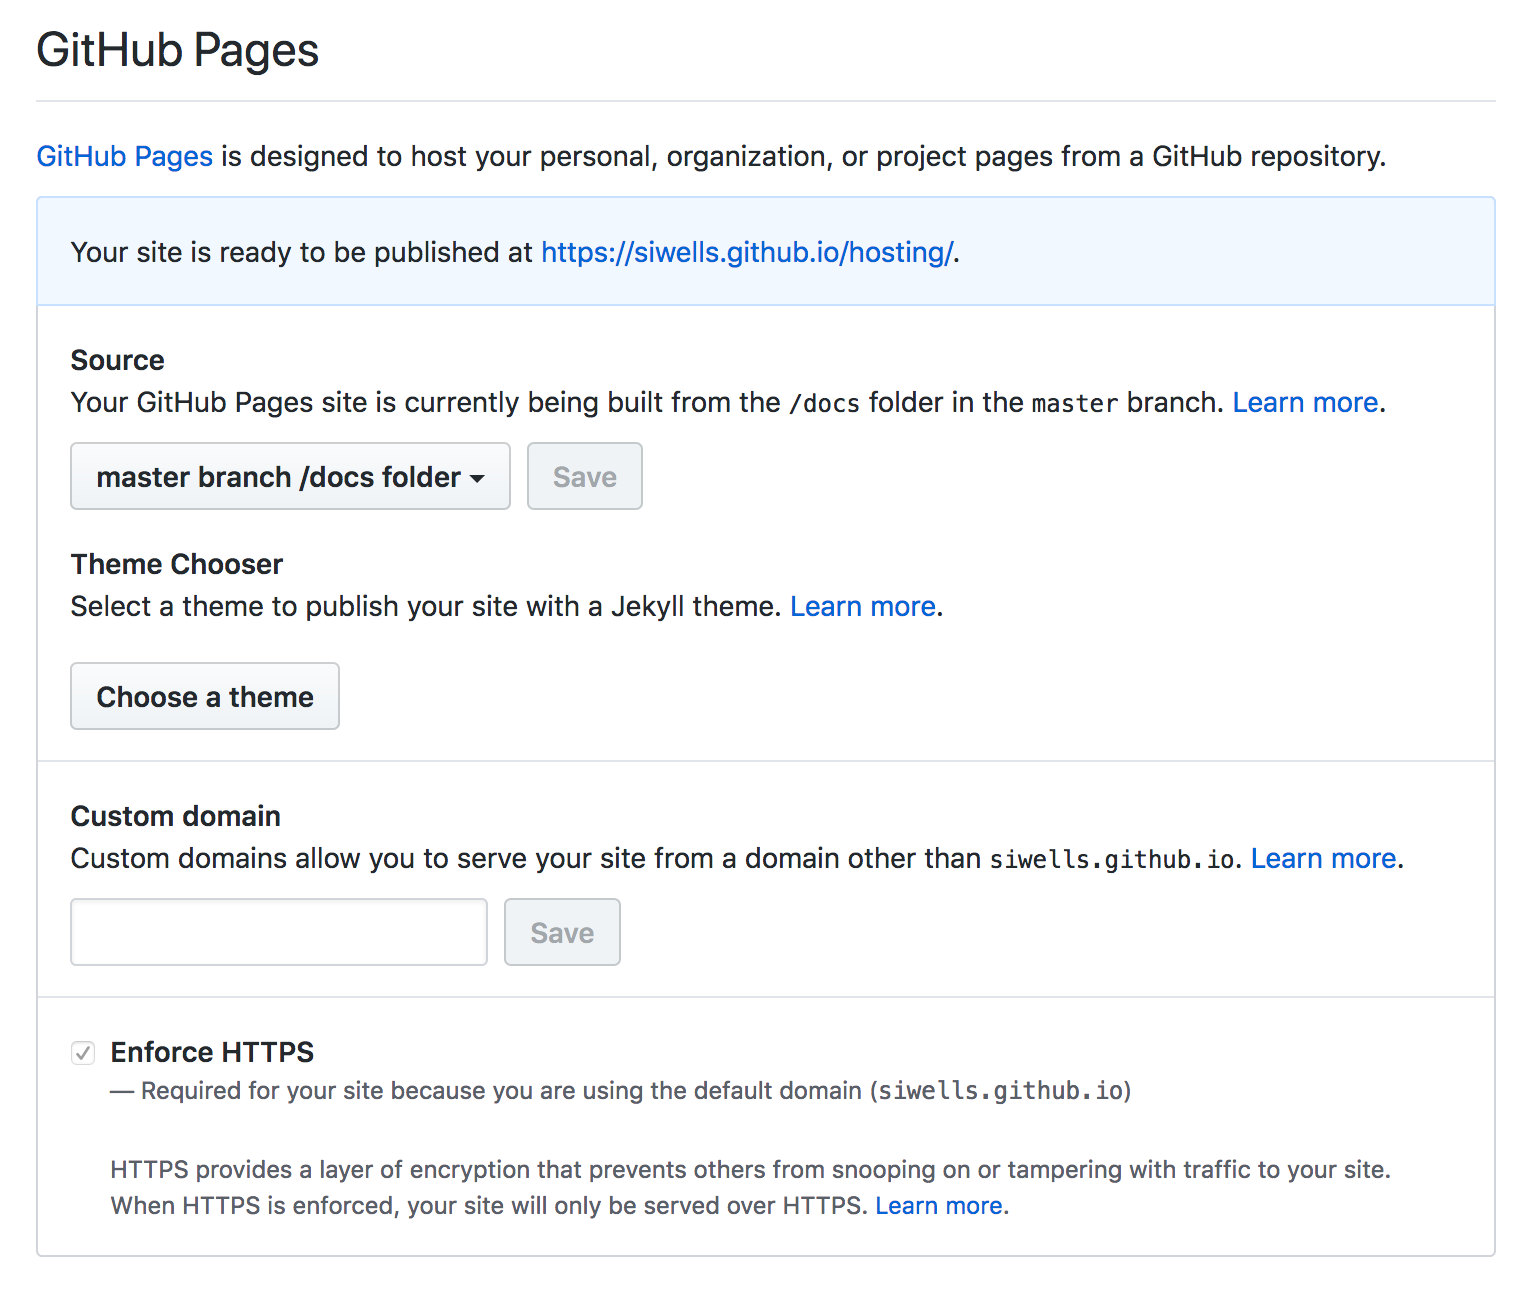
\includegraphics[width=0.85\textwidth]{images/github_config_after}
\caption{The GitHub config pages after enabling pages.}
\label{fig:github_config_after}
\end{figure}


\paragraph{} There are additional things you can do, like adding a custom domain name but that is beyond the scope of this lab\footnote{but again, that's something to add to your lists of things to explore.}. GitHub might take a few moments, but in theory you should now be able to navigate to your index.html in the docs folder and see it displayed as a regular webpage. GitHub should show you the address for your new site in the GitHub Pages section of the config. For example, my demo address was hosted at \url{https://siwells.github.io/hosting/} because I named my repository `hosting' and my GitHub account name is `siwells'. Anyway, navigate to the URL of your repository's pages and you should see something like this:

\begin{figure}[H]
\centering
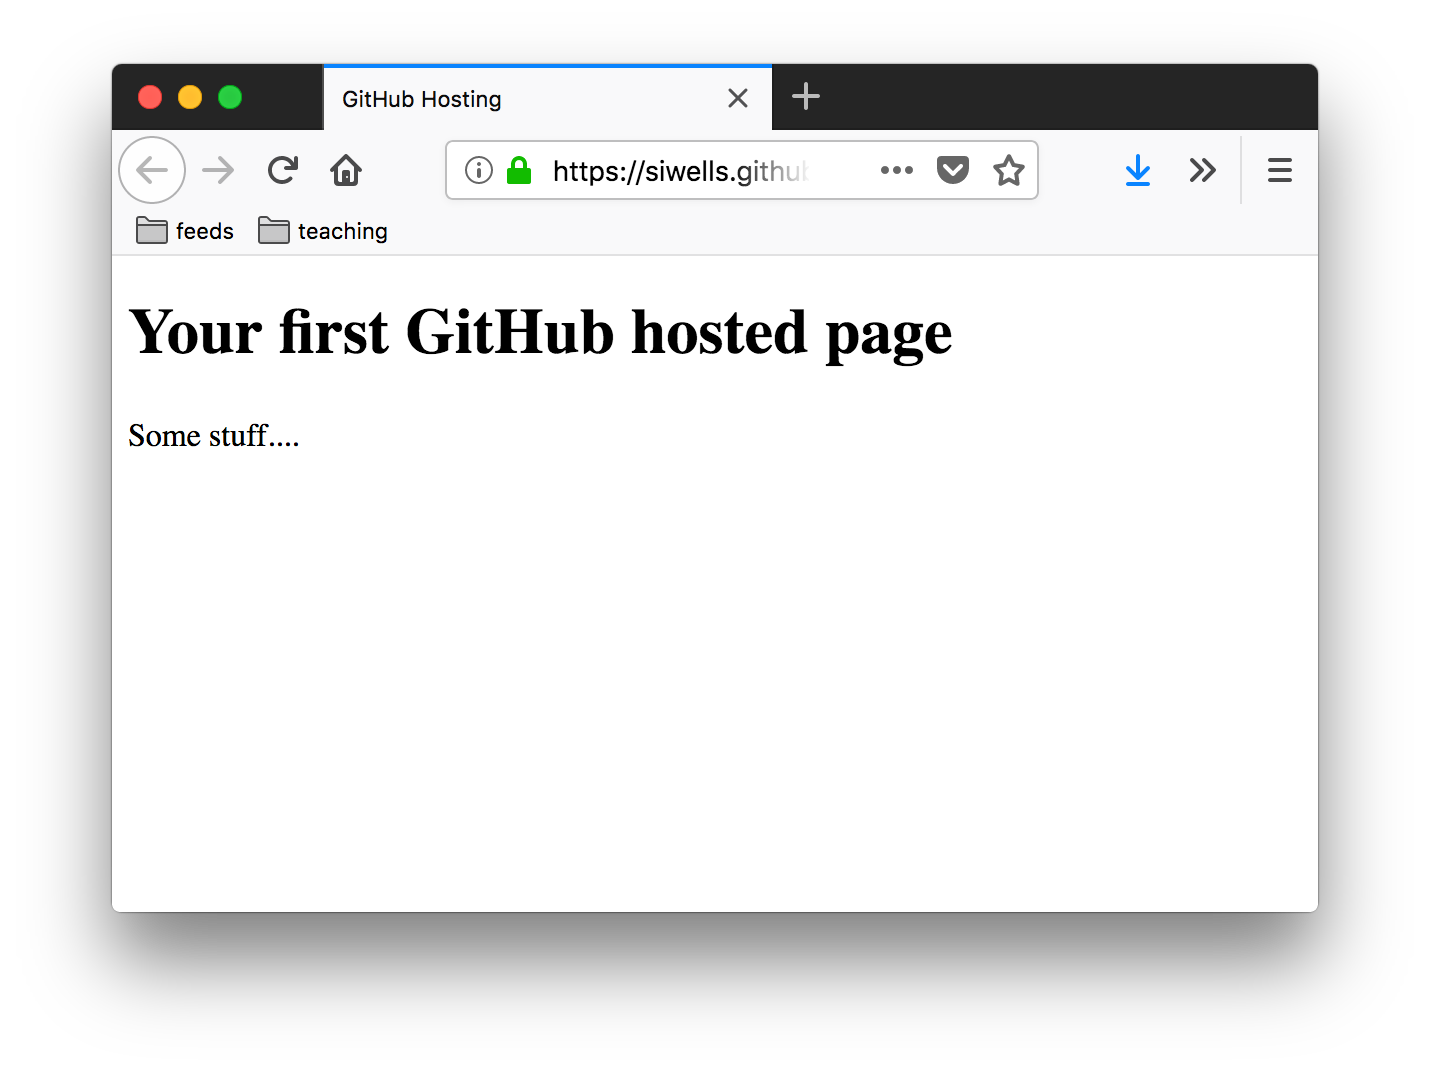
\includegraphics[width=0.85\textwidth]{images/github_hello}
\caption{Our GitHub hosted web page.}
\label{fig:github_hello}
\end{figure}

\paragraph{} There are many other free web hosting services as well as many paid services. Generally the paid services will offer more features and better reliability, but free services are a good place to start. Once you know you have enough users to need something better, then it's worth paying for. Although perhaps it's worth working out a way to provide some form of revenue. Try searching for web hosting services and get a feel for prices and services.

\section{Virtual Servers}
\paragraph{} Many places offer hosting services but often this is at the cost of running the software that the hosting provider specified. The next tier up is to run your own virtual server. This gives you much greater control over the software that runs, but requires more expertise to keep the server running both robustly and securely. For example, Linode are a popular and well priced solution \url{https://www.linode.com/pricing}. There are many others, e.g. at the time of writing, the following were the top results for a quick search on ``VPS'':

\begin{itemize}
\item \url{https://www.ovh.co.uk/vps/}
\item \url{https://www.vps.net/}
\item \url{https://uk.godaddy.com/hosting/vps-hosting}
\item \url{https://www.1and1.co.uk/virtual-server}
\end{itemize}

\paragraph{} There are also many providers who also offer free tiers to try out their services. These are generally very low performance, but are more than adequate for testing your deployment before spending any money.  You'll have to look around to find them though as these lowest tier machines are often used to hook in new customers through special offers.

\paragraph{} Spend some time investigating the range of web hosting provders and compariing facilities.

\end{document}

%\begin{framed}
%\end{framed}


%\begin{lstlisting}
%\end{lstlisting}

%\begin{lstlisting}[style=DOS]
%\end{lstlisting}
